\maketitle

\section*{Instructions}
Show all work and simplify final answers. You may use a calculator for arithmetic only.

\section*{Problems}
\begin{enumerate}
  \item Compute the limit, or state that it does not exist.
  \[\lim_{x \to 2} \frac{x^2 - 4}{x-2}\]
  \vspace{1.5in}

  \item Find the derivative of the function.
  \[f(x) = x^3 \ln(x) - \frac{4}{x^2}\]

  \newpage

  \item Compute the definite integral and sketch $y = 3x^2 - 4x + 1$ with the area for the integral shaded.
  \[\int_{0}^{2} (3x^2 - 4x + 1)\,dx\]

  \newpage

  \item Let $f(t)$ be defined by
  \[
    f(t) =
    \begin{cases}
      2 & 0 \le t < 2,\\
      2 - t & 2 \le t < 4,\\
      t - 4 & 4 \le t \le 6.
    \end{cases}
  \]
  Define
  \[F(x) = \int_{0}^{x} f(t)\,dt.\]
  On the axes below, sketch the graph of $F(x)$ for $0 \le x \le 6$.

  \begin{center}
    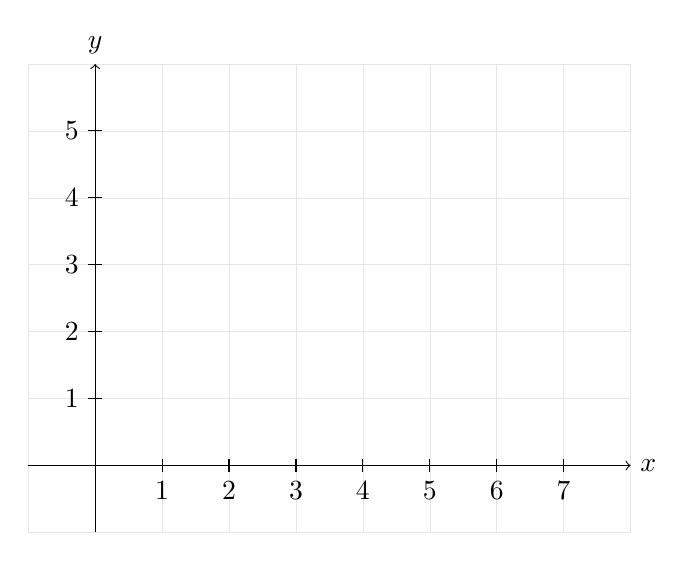
\begin{tikzpicture}[scale=0.85]
      \draw[step=1cm,gray!20,very thin] (-1,-1) grid (8,6);
      \draw[->] (-1,0) -- (8,0) node[right] {$x$};
      \draw[->] (0,-1) -- (0,6) node[above] {$y$};
      \foreach \x in {1,2,3,4,5,6,7}
        \draw (\x,0.1) -- (\x,-0.1) node[below] {\x};
      \foreach \y in {1,2,3,4,5}
        \draw (0.1,\y) -- (-0.1,\y) node[left] {\y};
    \end{tikzpicture}
  \end{center}
  \vspace{1.0in}

  \item Use the Fundamental Theorem of Calculus to find the derivative.
  \[G(x) = \int_{1}^{x} \sqrt{1 + t^4}\,dt\]
  \vspace{1.3in}
\end{enumerate}
